\section{Task structure in Fourier filtering}
\label{app:fourier-control}

\subsection{Full-family projection is an orbit average}

Write a Fourier mode as $\chi_{k,l}(a,b)=\exp(2\pi i(ka+lb)/p)$. Averaging its translations gives
\begin{equation}
\frac{1}{p}\sum_{t=0}^{p-1}\chi_{k,l}(a+t,b-t)
=\chi_{k,l}(a,b)\frac{1}{p}\sum_{t=0}^{p-1}\exp\!\left(\frac{2\pi i(k-l)t}{p}\right)
=\mathbf{1}_{k=l}\chi_{k,l}(a,b).
\end{equation}
Linearity proves Eq.~\ref{eq:orbit-average} for each feature channel. The surviving modes include $(0,0)$. For subtraction, averaging $(a+t,b+t)$ instead retains $k+l=0$ modulo $p$. With a linear head, $W_U P h=P(W_U h)$; an affine head also commutes with this average because averaging preserves its constant bias. Excluding the constant mode gives the orbit average minus the global mean.

The full-family filter therefore supplies the equivalence relation defining the answer. It can pool logits from training and held-out examples with that answer. This is part of the intervention itself, even though no labels are passed to the FFT routine. Its accuracy measures an answer-conditioned average and requires separate evidence to identify the algorithm implemented by the unfiltered model.

\subsection{A lookup-table memorizer}

We use the repository's five seeded splits, each with $3{,}830$ training and $8{,}939$ held-out examples at $p=113$. Let $T$ denote the training set and $e_s$ the one-hot vector for class $s$. The predictor stores $z(a,b)=e_{a+b}$ on $T$ and outputs zero on every unseen pair. If $n_s$ is the number of training examples with sum $s$,
\begin{equation}
(P_{\mathrm{add}}z)(a,b)=\frac{n_{a+b}}{p}e_{a+b}.
\end{equation}
Every answer orbit is covered in each split, so filtering yields $100\%$ accuracy. For a uniform split of $m=3{,}830$ out of $N=p^2$ pairs, an orbit is uncovered with probability $q=\binom{N-p}{m}/\binom{N}{m}$. A union bound gives $\Pr(\text{some orbit uncovered})\leq pq<2.89\times10^{-16}$. Before filtering, all held-out logits are tied. We use the smallest class index as the deterministic tie rule, matching the implementation's argmax; uniform random tie breaking has expected accuracy $1/113=0.885\%$.

\begin{table}[htbp]
\centering\small
\caption{Addition memorizer on the original seeded splits. Correct counts use the $8{,}939$ held-out examples. The filtered logits have a unique correct maximum on every example.}
\label{tab:memorizer}
\begin{tabular}{lrrrr}
\toprule
Seed & Raw correct & Raw accuracy (\%) & Filtered correct & Filtered accuracy (\%) \\
\midrule
$0$ & $79$ & $0.884$ & $8{,}939$ & $100.000$ \\
$1$ & $68$ & $0.761$ & $8{,}939$ & $100.000$ \\
$2$ & $79$ & $0.884$ & $8{,}939$ & $100.000$ \\
$3$ & $81$ & $0.906$ & $8{,}939$ & $100.000$ \\
$4$ & $77$ & $0.861$ & $8{,}939$ & $100.000$ \\
\bottomrule
\end{tabular}
\end{table}

The same control on subtraction reaches $100\%$ after the corresponding filter in all five seeds. Omitting the constant mode also retains perfect accuracy in these controls. A seeded bijection of output labels preserves the perfect filtered result when evaluated against those relabeled classes, because the projection still pools within answer orbits. Averaging training donors alone is sufficient; averaging only held-out donors gives zero logits for the memorizer.

These controls establish that full-family filtered accuracy can be perfect without a learned generalizing arithmetic algorithm. The $95.14\%$ filtered accuracy at AdamW step $3{,}000$ therefore requires independent evidence to establish when an internal arithmetic algorithm was learned. Evidence for surviving information at the collapsed checkpoints comes from the raw-feature decoder tests and adjacent-state swaps in \S\ref{sec:branches}.

\begin{figure}[t]
\centering
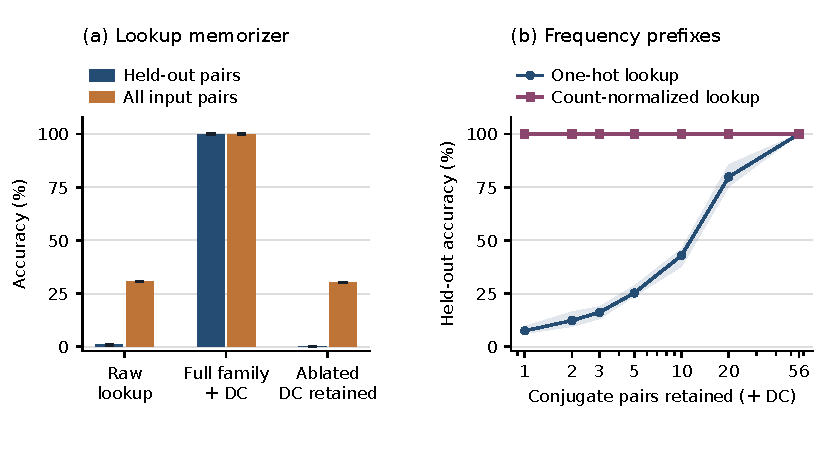
\includegraphics[width=\textwidth]{fourier_memorizer_control.pdf}
\caption{Task structure supplied by Fourier filtering at $p=113$. \textbf{(a)} The lookup memorizes the $3{,}830$ training answers and returns zero on the $8{,}939$ held-out inputs. Full-family filtering with DC gives $100\%$ accuracy. Family ablation retains DC and yields $0\%$ held-out accuracy and $29.99\%$ full-grid accuracy. Bars show means over five splits; whiskers span their range. \textbf{(b)} Training-count normalization allows any one diagonal conjugate pair plus DC to classify every input correctly. The ordinary lookup's pair powers are mathematically tied; its prefixes use increasing frequency as a fixed tie break. Lines show means and shading spans the seed range.}
\label{fig:fourier-memorizer}
\end{figure}

\subsection{Sparse sufficiency, ablation, and perturbation controls}

A second lookup stores $(p/n_c)e_c$ for a training example with label $c$, using training-label counts only, and zero for unseen pairs. Its full projection is exactly $e_{a+b}$. Retaining any one nonzero diagonal conjugate pair and DC gives class-$c$ logits
\begin{equation}
z_k(s,c)=\frac{1+2\cos(2\pi k(s-c)/p)}{p},\qquad s=(a+b)\bmod p.
\end{equation}
For prime $p=113$ and nonzero $k$, the unique maximum is at $c=s$. All $56$ individual pairs give $100\%$ training, held-out, and full-grid accuracy on all five splits ($280$ checks against the closed form). Thus sparse filtered sufficiency also admits a lookup-only predictor. The construction can use a $113$-dimensional lookup representation with an identity head, padded to the transformer's $128$-dimensional residual width.

The ordinary one-hot lookup has equal mathematical power in all diagonal conjugate pairs. With a fixed ascending-frequency tie break, five-pair filtering gives $23.82$--$28.57\%$ held-out accuracy; sorting the numerically computed powers instead gives $63.69$--$87.46\%$. These ranges expose the sensitivity of the selected frequencies to floating-point tie breaking in this control. Figure~\ref{fig:fourier-memorizer} uses the fixed ordering. The count-normalized lookup reaches $100\%$ at every tested prefix size $1,2,3,5,10,20,56$.

The original family-ablation convention is $z-Pz+\bar z$, retaining DC. For both lookups, it preserves all training predictions and gives $0\%$ held-out accuracy, hence $3{,}830/12{,}769=29.9945\%$ full-grid accuracy. The trained models' near-chance full-grid ablations in Table~\ref{tab:swap} contain additional information absent from this simple control. Full-family sufficiency and low held-out ablation accuracy can nevertheless occur together under memorization.

We also apply $20$ fixed-seed replicates per split and lookup for pair-global phases, channelwise phases, and derangements of the $56$ pair coefficients, preserving DC, conjugate symmetry, and total nonconstant family power. For the ordinary lookup, mean held-out accuracies of the isolated family are $1.0755\%$, $0.9426\%$, and $3.0680\%$, respectively; for the count-normalized lookup they are $0\%$, $0.8850\%$, and $3.1555\%$. Each mean pools $20$ perturbations per split across five splits; raw replicate distributions are released. The sensitivity observed in the trained models remains a functional measurement of their projected components. These controls show why that sensitivity alone leaves the internal algorithm unidentified.

\subsection{Restricting the averaging donors at captured failures}

Using both endpoints of the five adjacent failure pairs in Table~\ref{tab:adjacent}, we recompute logits from the saved raw residuals and native heads, multiplying in float64. We average only held-out inputs with the same answer, excluding the evaluated input itself. This removes both training donors and self contribution. Input order, labels, and masks are checked against the original seeded splits.

\begin{table}[htbp]
\centering\small
\caption{Held-out accuracy (\%) before and after each captured update. ``Average'' uses held-out donors with the same answer and excludes the evaluated example. The operation still supplies the grouping.}
\label{tab:fourier-donors}
\begin{tabular}{lrrrr}
\toprule
 & \multicolumn{2}{c}{Before} & \multicolumn{2}{c}{After} \\
Seed & Raw & Average & Raw & Average \\
\midrule
$0$ & $95.49$ & $100.00$ & $31.87$ & $30.46$ \\
$1$ & $94.14$ & $100.00$ & $9.09$ & $0.93$ \\
$2$ & $99.99$ & $100.00$ & $0.93$ & $0.88$ \\
$3$ & $89.54$ & $99.12$ & $53.60$ & $65.29$ \\
$4$ & $91.34$ & $98.18$ & $66.33$ & $71.25$ \\
\bottomrule
\end{tabular}
\end{table}

Before these updates, high accuracy survives removal of training donors, establishing task-aligned signal in the logits of unseen examples beyond the ordinary lookup control. The donor-restricted operation still uses the answer orbits and remains a task-informed diagnostic. These checkpoints are distinct from the early AdamW checkpoint at step $3{,}000$; this analysis makes no claim about its donor dependence.

Independent FFT, translated-grid sums, and orbit reductions agree in float64 at moduli $7$ and $113$. We also check projector idempotence, constant-mode conventions, readout commutation, coverage of every answer orbit, and the single-pair closed form. All scripts, protocols, integer counts, perturbation outcomes, and input hashes accompany the release.
